\section{Task Order in a Stateful Evaluation}
\label{sec:formulation}
Let $\pi$ denote a permutation of benchmark tasks. A memory-based agent maintains persistent state $M_t$ that is updated after task $t$. A stateful benchmark maintains environment state $E_t$, such as the order database behind a shopping website. Executing task $i$ with action trajectory $a_i$ induces
\begin{align}
M_{t+1} &= U_M(M_t,x_i,a_i,y_i),\\
E_{t+1} &= U_E(E_t,a_i),
\end{align}
where $x_i$ is the task and $y_i$ is observed feedback. Under order $\pi$, the score for task $i$ is
\begin{equation}
Y_i(\pi)=F\!\left(M_{<i}(\pi),E_{<i}(\pi),x_i,G_i\right),
\label{eq:joint}
\end{equation}
where $G_i$ is the evaluator. A memory-history estimand requires the compared orders to preserve the same environment path, $E(\pi_1)\equiv E(\pi_0)$. A live-state evaluator can achieve the same identification goal by deriving $G_i$ from the environment reached at execution time.

Figure~\ref{fig:causal} exposes the hidden causal path. The order intervention reaches the score through memory history and through environment history. Fixed reference text introduces an additional failure mode when it continues to describe an earlier service state.

\begin{figure}[t]
\centering
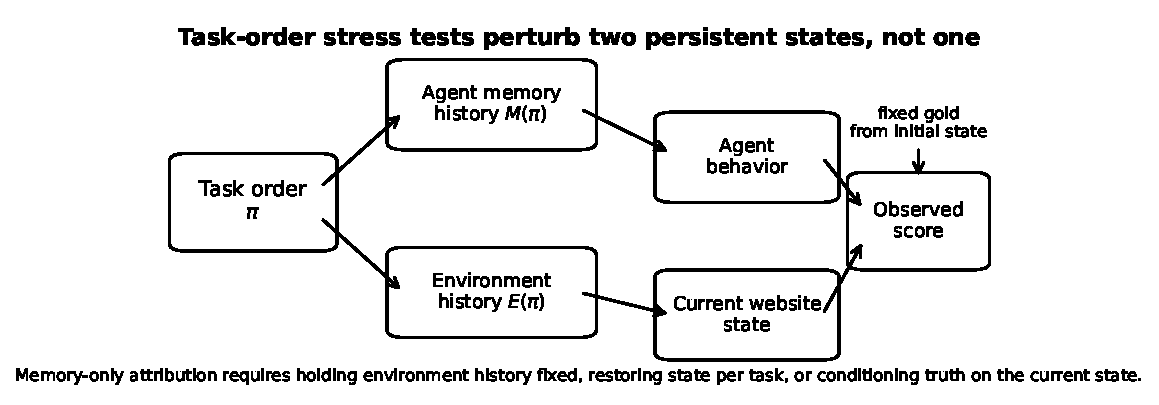
\includegraphics[width=\linewidth]{figures/fig1_causal_decomposition.pdf}
\caption{Task order jointly intervenes on the self-improving agent and the stateful benchmark. A clean memory-history estimate controls the environment-history path.}
\label{fig:causal}
\end{figure}

A fresh browser context does not restore a functional service database. The browser can restart while earlier purchases remain in the shopping backend. The relevant experimental state is therefore the persistent service state reached by previous benchmark tasks.
